\section{实验结果及分析}

\subsection{ALU验证实验结果}

ALU验证实验将B端口固定为32'h01，A端口依次输入不同的测试值，验证6种运算功能的正确性。实验结果如表~\ref{tab:alu_result}所示。

\begin{table}[htbp]
    \centering
    \begin{tabular}{c|c|c|c}
        操作 & F[2:0] & Num1 (A) & Result \\
        \hline
        A + B (Unsigned) & 000 & 32'h00000002 & 32'h00000003 \\
        A - B            & 001 & 32'h000000FF & 32'h000000FE \\
        A AND B          & 010 & 32'h000000FE & 32'h00000000 \\
        A OR B           & 011 & 32'h000000AA & 32'h000000AB \\
        $\overline{A}$   & 100 & 32'h000000F0 & 32'hFFFFFF0F \\
        SLT              & 101 & 32'h00000081 & 32'h00000000 \\
        \hline
    \end{tabular}
    \caption{ALU验证结果表}
    \label{tab:alu_result}
\end{table}

\textbf{结果分析：}
\begin{enumerate}
    \item \textbf{A+B (Unsigned)}：0x00000002 + 0x00000001 = 0x00000003，结果正确
    \item \textbf{A - B}：0x000000FF - 0x00000001 = 0x000000FE，结果正确
    \item \textbf{A AND B}：0x000000FE \& 0x00000001 = 0x00000000，结果正确
    \item \textbf{A OR B}：0x000000AA $\vert$ 0x00000001 = 0x000000AB，结果正确
    \item \textbf{NOT A}：\textasciitilde 0x000000F0 = 0xFFFFFF0F，结果正确
    \item \textbf{SLT}：\$signed(0x00000081) = 129，\$signed(0x00000001) = 1，129 < 1 为假，输出0，结果正确
\end{enumerate}

\subsection{流水线阻塞仿真图}

仿真中前10个周期正常进行加法运算，输入数据依次为0x11110000+0x22220000、0x22220000+0x33330000等。第10个时钟周期后，stall信号拉高并持续2个周期。stall有效期间，流水线所有寄存器保持原值不变，新的输入数据无法进入流水线。2个周期后stall信号拉低，流水线恢复正常流动。

\begin{figure}[htbp]
    \centering
    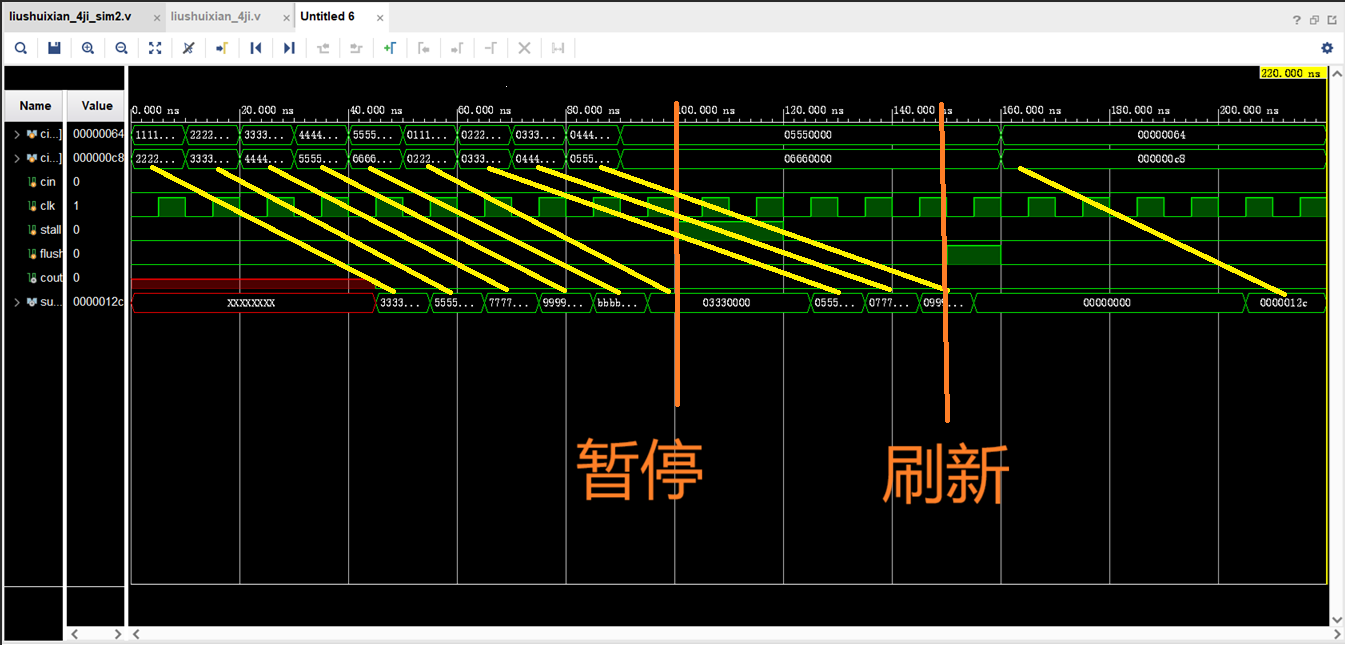
\includegraphics[width=0.95\textwidth]{image/pipeline_sim.png}
    \caption{流水线暂停仿真波形图}
    \label{fig:pipe_stall}
\end{figure}

\subsection{流水线刷新仿真图}

stall结束后继续正常运算。第15个时钟周期时，flush信号拉高并持续1个周期。flush有效期间，流水线所有寄存器被清零，包括各级部分和、进位、剩余数据以及移位寄存器。flush结束后，流水线从零状态重新开始流动，后续输入0x64+0xC8正常运算出结果0x12C。
